% Options for packages loaded elsewhere
\PassOptionsToPackage{unicode}{hyperref}
\PassOptionsToPackage{hyphens}{url}
%
\documentclass[
]{book}
\usepackage{amsmath,amssymb}
\usepackage{iftex}
\ifPDFTeX
  \usepackage[T1]{fontenc}
  \usepackage[utf8]{inputenc}
  \usepackage{textcomp} % provide euro and other symbols
\else % if luatex or xetex
  \usepackage{unicode-math} % this also loads fontspec
  \defaultfontfeatures{Scale=MatchLowercase}
  \defaultfontfeatures[\rmfamily]{Ligatures=TeX,Scale=1}
\fi
\usepackage{lmodern}
\ifPDFTeX\else
  % xetex/luatex font selection
\fi
% Use upquote if available, for straight quotes in verbatim environments
\IfFileExists{upquote.sty}{\usepackage{upquote}}{}
\IfFileExists{microtype.sty}{% use microtype if available
  \usepackage[]{microtype}
  \UseMicrotypeSet[protrusion]{basicmath} % disable protrusion for tt fonts
}{}
\makeatletter
\@ifundefined{KOMAClassName}{% if non-KOMA class
  \IfFileExists{parskip.sty}{%
    \usepackage{parskip}
  }{% else
    \setlength{\parindent}{0pt}
    \setlength{\parskip}{6pt plus 2pt minus 1pt}}
}{% if KOMA class
  \KOMAoptions{parskip=half}}
\makeatother
\usepackage{xcolor}
\usepackage{color}
\usepackage{fancyvrb}
\newcommand{\VerbBar}{|}
\newcommand{\VERB}{\Verb[commandchars=\\\{\}]}
\DefineVerbatimEnvironment{Highlighting}{Verbatim}{commandchars=\\\{\}}
% Add ',fontsize=\small' for more characters per line
\usepackage{framed}
\definecolor{shadecolor}{RGB}{248,248,248}
\newenvironment{Shaded}{\begin{snugshade}}{\end{snugshade}}
\newcommand{\AlertTok}[1]{\textcolor[rgb]{0.94,0.16,0.16}{#1}}
\newcommand{\AnnotationTok}[1]{\textcolor[rgb]{0.56,0.35,0.01}{\textbf{\textit{#1}}}}
\newcommand{\AttributeTok}[1]{\textcolor[rgb]{0.13,0.29,0.53}{#1}}
\newcommand{\BaseNTok}[1]{\textcolor[rgb]{0.00,0.00,0.81}{#1}}
\newcommand{\BuiltInTok}[1]{#1}
\newcommand{\CharTok}[1]{\textcolor[rgb]{0.31,0.60,0.02}{#1}}
\newcommand{\CommentTok}[1]{\textcolor[rgb]{0.56,0.35,0.01}{\textit{#1}}}
\newcommand{\CommentVarTok}[1]{\textcolor[rgb]{0.56,0.35,0.01}{\textbf{\textit{#1}}}}
\newcommand{\ConstantTok}[1]{\textcolor[rgb]{0.56,0.35,0.01}{#1}}
\newcommand{\ControlFlowTok}[1]{\textcolor[rgb]{0.13,0.29,0.53}{\textbf{#1}}}
\newcommand{\DataTypeTok}[1]{\textcolor[rgb]{0.13,0.29,0.53}{#1}}
\newcommand{\DecValTok}[1]{\textcolor[rgb]{0.00,0.00,0.81}{#1}}
\newcommand{\DocumentationTok}[1]{\textcolor[rgb]{0.56,0.35,0.01}{\textbf{\textit{#1}}}}
\newcommand{\ErrorTok}[1]{\textcolor[rgb]{0.64,0.00,0.00}{\textbf{#1}}}
\newcommand{\ExtensionTok}[1]{#1}
\newcommand{\FloatTok}[1]{\textcolor[rgb]{0.00,0.00,0.81}{#1}}
\newcommand{\FunctionTok}[1]{\textcolor[rgb]{0.13,0.29,0.53}{\textbf{#1}}}
\newcommand{\ImportTok}[1]{#1}
\newcommand{\InformationTok}[1]{\textcolor[rgb]{0.56,0.35,0.01}{\textbf{\textit{#1}}}}
\newcommand{\KeywordTok}[1]{\textcolor[rgb]{0.13,0.29,0.53}{\textbf{#1}}}
\newcommand{\NormalTok}[1]{#1}
\newcommand{\OperatorTok}[1]{\textcolor[rgb]{0.81,0.36,0.00}{\textbf{#1}}}
\newcommand{\OtherTok}[1]{\textcolor[rgb]{0.56,0.35,0.01}{#1}}
\newcommand{\PreprocessorTok}[1]{\textcolor[rgb]{0.56,0.35,0.01}{\textit{#1}}}
\newcommand{\RegionMarkerTok}[1]{#1}
\newcommand{\SpecialCharTok}[1]{\textcolor[rgb]{0.81,0.36,0.00}{\textbf{#1}}}
\newcommand{\SpecialStringTok}[1]{\textcolor[rgb]{0.31,0.60,0.02}{#1}}
\newcommand{\StringTok}[1]{\textcolor[rgb]{0.31,0.60,0.02}{#1}}
\newcommand{\VariableTok}[1]{\textcolor[rgb]{0.00,0.00,0.00}{#1}}
\newcommand{\VerbatimStringTok}[1]{\textcolor[rgb]{0.31,0.60,0.02}{#1}}
\newcommand{\WarningTok}[1]{\textcolor[rgb]{0.56,0.35,0.01}{\textbf{\textit{#1}}}}
\usepackage{longtable,booktabs,array}
\usepackage{calc} % for calculating minipage widths
% Correct order of tables after \paragraph or \subparagraph
\usepackage{etoolbox}
\makeatletter
\patchcmd\longtable{\par}{\if@noskipsec\mbox{}\fi\par}{}{}
\makeatother
% Allow footnotes in longtable head/foot
\IfFileExists{footnotehyper.sty}{\usepackage{footnotehyper}}{\usepackage{footnote}}
\makesavenoteenv{longtable}
\usepackage{graphicx}
\makeatletter
\def\maxwidth{\ifdim\Gin@nat@width>\linewidth\linewidth\else\Gin@nat@width\fi}
\def\maxheight{\ifdim\Gin@nat@height>\textheight\textheight\else\Gin@nat@height\fi}
\makeatother
% Scale images if necessary, so that they will not overflow the page
% margins by default, and it is still possible to overwrite the defaults
% using explicit options in \includegraphics[width, height, ...]{}
\setkeys{Gin}{width=\maxwidth,height=\maxheight,keepaspectratio}
% Set default figure placement to htbp
\makeatletter
\def\fps@figure{htbp}
\makeatother
\setlength{\emergencystretch}{3em} % prevent overfull lines
\providecommand{\tightlist}{%
  \setlength{\itemsep}{0pt}\setlength{\parskip}{0pt}}
\setcounter{secnumdepth}{5}
\usepackage{booktabs}
\ifLuaTeX
  \usepackage{selnolig}  % disable illegal ligatures
\fi
\usepackage[]{natbib}
\bibliographystyle{plainnat}
\IfFileExists{bookmark.sty}{\usepackage{bookmark}}{\usepackage{hyperref}}
\IfFileExists{xurl.sty}{\usepackage{xurl}}{} % add URL line breaks if available
\urlstyle{same}
\hypersetup{
  pdftitle={render book},
  pdfauthor={ML},
  hidelinks,
  pdfcreator={LaTeX via pandoc}}

\title{render book}
\author{ML}
\date{2024-01-06}

\usepackage{amsthm}
\newtheorem{theorem}{Theorem}[chapter]
\newtheorem{lemma}{Lemma}[chapter]
\newtheorem{corollary}{Corollary}[chapter]
\newtheorem{proposition}{Proposition}[chapter]
\newtheorem{conjecture}{Conjecture}[chapter]
\theoremstyle{definition}
\newtheorem{definition}{Definition}[chapter]
\theoremstyle{definition}
\newtheorem{example}{Example}[chapter]
\theoremstyle{definition}
\newtheorem{exercise}{Exercise}[chapter]
\theoremstyle{definition}
\newtheorem{hypothesis}{Hypothesis}[chapter]
\theoremstyle{remark}
\newtheorem*{remark}{Remark}
\newtheorem*{solution}{Solution}
\begin{document}
\maketitle

{
\setcounter{tocdepth}{1}
\tableofcontents
}
\hypertarget{preface}{%
\chapter{Preface}\label{preface}}


In this book, we aim at understanding some powers of music with the help of statistical modelling.
Thanks to recent developments in measuring, high-dimensional synchronized data streams become available in big quantities. Typically, they contain streams of audio, body movement and brain activity, all nicely synchronized during interactions driven by music, such as during listening, dancing, music performing tasks, either individually or in a group together with friends.
The goal is to understand what these interactions bring about and why people tend to see music as a positive power affecting them.

However, despite recent progress, the power of music remains much of a mystery.
Fine-grained measurements can be done but the gap between theory and data remains challenging.
Hence this book.
The book is about statistical modelling in view of understanding how music affects humans. It is conceived -- not as a textbook -- but as a bridge between theory and data, to close the gap between theory and data.

\hypertarget{limitations}{%
\section{Limitations}\label{limitations}}

Despite the broad claim of understanding the power of music, we focus on limited topics, contributing small steps to a global ambition of understanding. The title of the book says \(some powers of music\), just to make sure that there is no misunderstanding of what we can.

Despite exciting developments in neurobiology and neuroscience, this book is also limited to the analysis of behavioral data using regression analysis, although other types of analysis are used as well.

Despite the belief that the effect of music is greatest in real-world contexts, we adopt a
theoretical framework that is rooted in cognitive science. The latter implies that in view of reliable data gathering, controlled contexts are defined in which interactions driven by music can be studied. This reduces the ecological validity, and its limitating. However, it allows for approaches that focus upon specific interaction processes (such as entrainment) and it allows for the use of specific technologies (such as virtual reality) that can break into the action-perception loops that govern the interactions.

Finally, we don't strive for an exhaustive account of statistical modelling techniques. Rather,
we focus on a limited range of (mainly regression) techniques that are deemed relevant for understanding data in view of a particular theory.

\hypertarget{overview}{%
\section{Overview}\label{overview}}

This book is devoted to case studies but it starts with a theoretical framework, presented in chapter \ref{chapTheory}. Theory is needed because it offers the reader a framework for understanding what empirical music research is about, and what we are aiming for when analyzing the data.
The theory is needed to interpret the data and see why certain statistical modelling techniques are relevant and other not.

The next chapter \ref{chapModelling} sketches a general methodological framework for statistical modelling and music. Examples are given of \emph{circular-linear} regression modelling, as a method to capture the temporal circularity of musical rhythms. These examples set the tone for further examples, explored in case studies.

We then proceed with the case studies.
Chapter \ref{chapListener} accesses the listener's music appreciation. There is nothing temporal, multi-model, nor multi-medial here. Yet questionnaires are valuable instruments for understanding the effect of music on humans, using \emph{structural equation modelling} as statistical modelling tool.

Chapter \ref{chapDancer}
is about the effect of repeated musical phrases on sensorimotor synchronization in classical ballet dancing. The chapter is an application of \emph{circular-linear regression modelling}, including an approach to contrast musical phrases.

Chapter \ref{chapViolinist}
is about the learning effect of a 3D versus 2D music play-along system for violin, for training synchronized bowing gestures in an orchestra.
To figure out the effect, \emph{hierarchical regression modelling} is used.

Chapter \ref{chapEntrainment} is about rhythmic entrainment in human dyads. The modelling is a bit more advanced in that it involves a system of ordinal differential equations (ODE-system) as predictor for \emph{time-dependent} data.

The last chapter offers some perspectives for future work in this field.

\hypertarget{usage}{%
\section{Usage}\label{usage}}

Each chapter can be read independently.
However, it is highly recommended to read the chapter on theory first.
It offers the overall framework for understanding specific research questions addressed in subsequent chapters.

Chapters contain code illustrations but the interested reader can consult the entire script for further details. The scripts are organized per chapter and processing.
A script has the following name-syntax: \texttt{script\_XXX\_YYY\_ZZZ.R}.
XXX indicates the shortname of a chapter, such as \texttt{chapListener}, \texttt{chapDancer}. These names are shortcuts for full chapter names.
YYY is a sequence number, which indicates the order in which the script should be processed.
ZZZ is a processing module, such as initialization, data processing, data plotting and so on.
For example, \texttt{script\_chapListener\_02\_DataPreparation.R} means: an R-script in the chapter on the listener, second in order (a script with 01 is about initialization and should be executed before 02), and about data preparation.
For example, \texttt{script\_chapListener\_05\_ModelPlotting.R} is about model plotting. It should be executed after running the modelling script \texttt{script\_chapListener\_04\_Modelling.R}. But that script requires at least that script 01 and 02 have been executed, possibly also 03.
The scripts that should be run in each chapter are called: \texttt{script\_chapAll\_01\_Initialization.R} and \texttt{script\_chapAll\_02\_Functions.R}.

\hypertarget{background}{%
\section{Background}\label{background}}

Sources of inspiration have been:
- John Kruschke \emph{Doing Bayesian data analysis}
- Richard McElreath's \emph{Rethinking statistics}
-
-
-
-.

\hypertarget{setting-up-your-computational-environment}{%
\section{Setting up your computational environment}\label{setting-up-your-computational-environment}}

As computational tool for statistical analysis, we use R and several R-packages in RStudio.
For regression modelling, we draw mainly on \texttt{lme4}, \texttt{brms}, and some own coding in STAN.

\hypertarget{chapViolinist}{%
\chapter{Understanding violin playing with a play-along}\label{chapViolinist}}

This chapter is about violin playing in an orchestra.
Imagine an orchestra and its string section. Typically, the members of the string section, the violinists, have their bow strokes going up and down in synchronized manner, so that they appear as one single organism moving together. Less experienced violinists have to learn to play in sync with the principal violinist of the section. They need to learn the bowing gestures as well as the particular expression associated with it.

To train these bowing gestures, it is possible to use an audiovisual play-along system with a visual representation of the principal violinist.
In this chapter we investigate the effect of a 2D or 3D representation of the principal violinist, based on Campo et al.~(2023).
Which condition is more effective for learning? The reader might guess that the 3D-avatar is better.

\hypertarget{theoretical-basis}{%
\section{Theoretical basis}\label{theoretical-basis}}

With this play-along, the student has to acquire bowing gestures aligned with a teacher-avatar.
It can be assumed that the observation of a teacher-avatar in 3D, through the Hololens, yields a more effective outcome compared to a teacher-avatar viewed in 2D, through the same Hololens. The rationale behind this assumption is rooted in the unique capabilities of the Hololens to allow for a changing point of view, enabling parallax when the avatar is in 3D. Accordingly, essential information can be obtained by active sampling through head movements of the student, enabling a more nuanced interpretation of the observed bowing gestures exhibited by the teacher. Based on this assumption, it is likely that the alignment of the student's bowing gestures with the teacher-avatar will be better in 3D than in 2D.

\hypertarget{metric}{%
\section{Metric}\label{metric}}

To test the assumption, it suffices to compare the student's bowing gestures with the teacher's bowing gestures. In Campo et al.~(2023) bowing gestures having been identified and isolated using techniques based on motion caption recordings. Once identified, bowing gestures of student and teacher can be compared using a similarity metric. Campo et al.~(2023) calculated the Procrustes Distance (PD), which quantifies the extent of deformation needed to transform one gesture into the other gesture. It is based on the scaling, rotating, and translating of the student's bowing gesture. Smaller PD values indicates greater similarity between bowing gestures.

\hypertarget{experiment}{%
\section{Experiment}\label{experiment}}

In this experiment, only eleven participants were recruited, all members from the UGent student orchestra GUSO.
They were engaged in four practice trials spaced evenly over the course of a month, with each participant experiencing both conditions (2D, 3D). Like in real orchestral playing, where members of the string section follow the principal violinist, participants were instructed to closely imitate the avatar's bowing gestures, encompassing bowings, articulations, and dynamics.

Due to the limited amount of participants the design is somewhat peculiar in the sense that
each participant takes part in two conditions (2D and 3D), with four trials per condition (T1, T2, T3, T4).
However, conditions apply to different pieces (F1, F2, F3, F4), with F1 and F2 for first violin players, and F3 and F4 for second violin players. The structure is shown in table @ref(tab:chapViolinist\_Design1).
This design does not allow us to check condition per subject and per piece.
However, for each piece, we can compare the groups per condition.
For example, for F1, we have P004-6-9 playing in 2D and we have P001-2-10 playing in 3D.
Those two groups can be compared.

\begin{Shaded}
\begin{Highlighting}[]
\FunctionTok{load}\NormalTok{(}\AttributeTok{file =} \StringTok{"Data/chapViolinistData.RData"}\NormalTok{)}

\NormalTok{D }\OtherTok{\textless{}{-}}\NormalTok{ Data }\SpecialCharTok{\%\textgreater{}\%} \FunctionTok{select}\NormalTok{(subject, condition, piece) }\SpecialCharTok{\%\textgreater{}\%} \FunctionTok{arrange}\NormalTok{(piece,condition) }\SpecialCharTok{\%\textgreater{}\%} \FunctionTok{unique}\NormalTok{()}
\FunctionTok{rownames}\NormalTok{(D) }\OtherTok{\textless{}{-}} \ConstantTok{NULL}
\NormalTok{D}
\end{Highlighting}
\end{Shaded}

\begin{verbatim}
##    subject condition piece
## 1     P004        2D    F1
## 2     P006        2D    F1
## 3     P009        2D    F1
## 4     P001        3D    F1
## 5     P002        3D    F1
## 6     P010        3D    F1
## 7     P001        2D    F2
## 8     P002        2D    F2
## 9     P010        2D    F2
## 10    P004        3D    F2
## 11    P006        3D    F2
## 12    P009        3D    F2
## 13    P003        2D    F3
## 14    P005        2D    F3
## 15    P007        3D    F3
## 16    P008        3D    F3
## 17    P011        3D    F3
## 18    P007        2D    F4
## 19    P008        2D    F4
## 20    P011        2D    F4
## 21    P003        3D    F4
## 22    P005        3D    F4
\end{verbatim}

\begin{Shaded}
\begin{Highlighting}[]
\CommentTok{\# \textbackslash{}@ref(tab:chapViolinist\_Design1)}
\end{Highlighting}
\end{Shaded}

Eleven subjects is not much. However, in music research it is often the case that we have few subjects participating in the experiment. The reason is that experiments are very time-consuming and that subjects are few and sometimes hard to find, especially for participation in longitudinal studies.
Nevertheless, thanks to repeated measures in four trials, we are just on the border of having enough statistical power.

\hypertarget{dataset-and-modelling}{%
\section{Dataset and modelling}\label{dataset-and-modelling}}

The study has been published in Campo et al.~(2023a). The dataset can be downloaded from Campo et al.~(2023b) and additional software is available at Campo et al.~(2024).
Here we focus on aspects of statistical modelling not explicitly contained in the above publications.
Two approaches will be developed.
The first approach is based on the groups.
The second approach is based on individual subjects.

The original dataset comprises motion capture, audio, and questionnaire data from violinists. Here we use the dataset specified in table @ref(tab:chapViolinist\_Design2).

\begin{verbatim}
## # A tibble: 6 x 9
##       PD logPD[,1] startIndex endIndex  time subject trial condition piece
##    <dbl>     <dbl>      <dbl>    <dbl> <dbl> <fct>   <fct> <fct>     <chr>
## 1 0.0916    -0.766       3.59     4.3   3.59 P001    T1    3D        F1   
## 2 0.0916    -0.766       3.59     4.3   3.89 P001    T1    3D        F1   
## 3 0.0916    -0.766       3.59     4.3   4.19 P001    T1    3D        F1   
## 4 0.210      0.409       4.3      5.33  4.3  P001    T1    3D        F1   
## 5 0.210      0.409       4.3      5.33  4.6  P001    T1    3D        F1   
## 6 0.210      0.409       4.3      5.33  4.9  P001    T1    3D        F1
\end{verbatim}

The first two columns contain the metrics of the Procustus Distance, \texttt{PD} and its logarithm \texttt{logPD}.
The columns \texttt{startIndex} and \texttt{endIndex} contain the start and end times of a bowing gesture in seconds.
The sampling rate of 3.3 sa/sec gives about one samples every 0.3 seconds.
The sample times are indicated in \texttt{time}.
The other columns \texttt{subject}, \texttt{trial}, \texttt{condition\textasciigrave{}\textasciigrave{},}piece` are factors having levels (11 subjects, 4 trials, 2 conditions, 4 pieces).

\hypertarget{data-plotting}{%
\section{Data plotting}\label{data-plotting}}

A histogram of all data of the PD metric, shown in the left panel of figure @ref(fig:chapViolinist\_PD\_hist), suggests a Poisson-like distribution of the PD values.
Basically, a good performance is a performance where the student's bow strokes are in sync with the teacher's bow strokes. The lower the PD, the more similar the bowing gesture resembles the teacher's bowing gesture. The right panel of figure @ref(fig:chapViolinist\_PD\_hist) shows the logarithmic transformation of the PD values. Low values get a bit more stretched, and high values get squeezed. The difference between conditions at higher values is a bit more clear. Moreover, the logPD will allow us to work with a gaussian or, as we did, a skewed normal, link function in the regression model.

\begin{figure}

{\centering \includegraphics[width=0.35\linewidth]{_main_files/figure-latex/chapViolinist_PD_hist-1} 

}

\caption{Density of PD for 2D and 3D}(\#fig:chapViolinist_PD_hist)
\end{figure}

Figure @ref(fig:chapViolinist\_PD\_data) shows the data as they evolve over time, with four different pieces (F1,F2,F3,F4) and two conditions (2D, 3D).
The vertical axis shows the logPD.
The horizontal axis shows the time.
Each dot represents a sample logPD value.

As mentioned, a bowing gesture has a duration corresponding to the duration of the played note(s). Accordingly, longer bowing gestures are represented as a sequence of dots having equal logPD.
The white gaps reveal silence (no bowing gesture).

\begin{figure}

{\centering \includegraphics[width=0.75\linewidth]{_main_files/figure-latex/chapViolinist_PD_data-1} 

}

\caption{Data of four pieces in two conditions}(\#fig:chapViolinist_PD_data)
\end{figure}

Some differences between 2D and 3D can be observed. For example, in the first column (piece F1), first row (condition 2D), there are quite some dots around zero in 2D, whereas almost no dots around zero in the second row (condition 3D). This suggests a better alignment in 3D. However, in the second column (piece F2) it looks as if the higher values logPD occur in 3D, compared to 2D, at least towards the end of the piece.

In what follows, the analysis procedure is fully explained with F1, the first piece. We then summarize the results for the other pieces.

\begin{figure}

{\centering \includegraphics[width=1\linewidth]{Figures/chapViolinist_F1_score} 

}

\caption{Data of four pieces in two conditions}(\#fig:chapViolinist_F1_score)
\end{figure}

\hypertarget{modelling}{%
\section{Modelling}\label{modelling}}

As mentioned we proceed along two tracks.
In the first approach, we use groups defined by condition within the piece F1.
The model syntax is defined in expression \eqref{eq:chapViolinistModel1}.
The \texttt{logPD} response is modeled by a general intercept (1), an intercept for the two levels of \texttt{condition}, and a smooth over \texttt{time} for the levels of \texttt{condition} (2D, 3D), as defined by a basis of 50 splines and regularization with \(m=2\).

\begin{equation}
\begin{matrix}
&logPD \sim 1 + condition +  s(time, by = condition, k = 50,m=2) + 
(1 | trial + subject)
\end{matrix}
\label{eq:chapViolinistModel1}
\end{equation}

In \texttt{brms}, it comes at a very high computational cost due to the algorithms for optimization based on monte carlo simulations (see McElreath, Kruschke). However, \texttt{brms} is more flexible than \texttt{mgcv}.
And once the model is calculated, a posterior prediction can be generated using a newly defined data grid in which time is sampled every .5 second and all other variables in the model are accordingly sampled
The prediction contains one \emph{posterior predictive distribution} per specified time point, and we can then easily contrast the distributions of the 2D and 3D condition and obtain the \emph{posterior difference distribution}.
When that posterior has its probability mass for 90\% above or below zero, it means that 2D and 3D can be considered to be different.
Note that we will have this posterior at each time instance, so that the performance in 2D versus 3D can be contrasted over time.
To summarize the steps: (i) run the regression model with a dataset of sampled bow strokes, (ii) generate a model-based prediction using a dataset with sampled time (e.g.~every .5 seconds), (iii) contrast 2D and 3D predictions at each sampled time, (iv) check pd (probability direction) at each sampled time.

\hypertarget{contrasts}{%
\section{Contrasts}\label{contrasts}}

\hypertarget{first-piece-f1}{%
\subsection{First piece (F1)}\label{first-piece-f1}}

\begin{figure}

{\centering 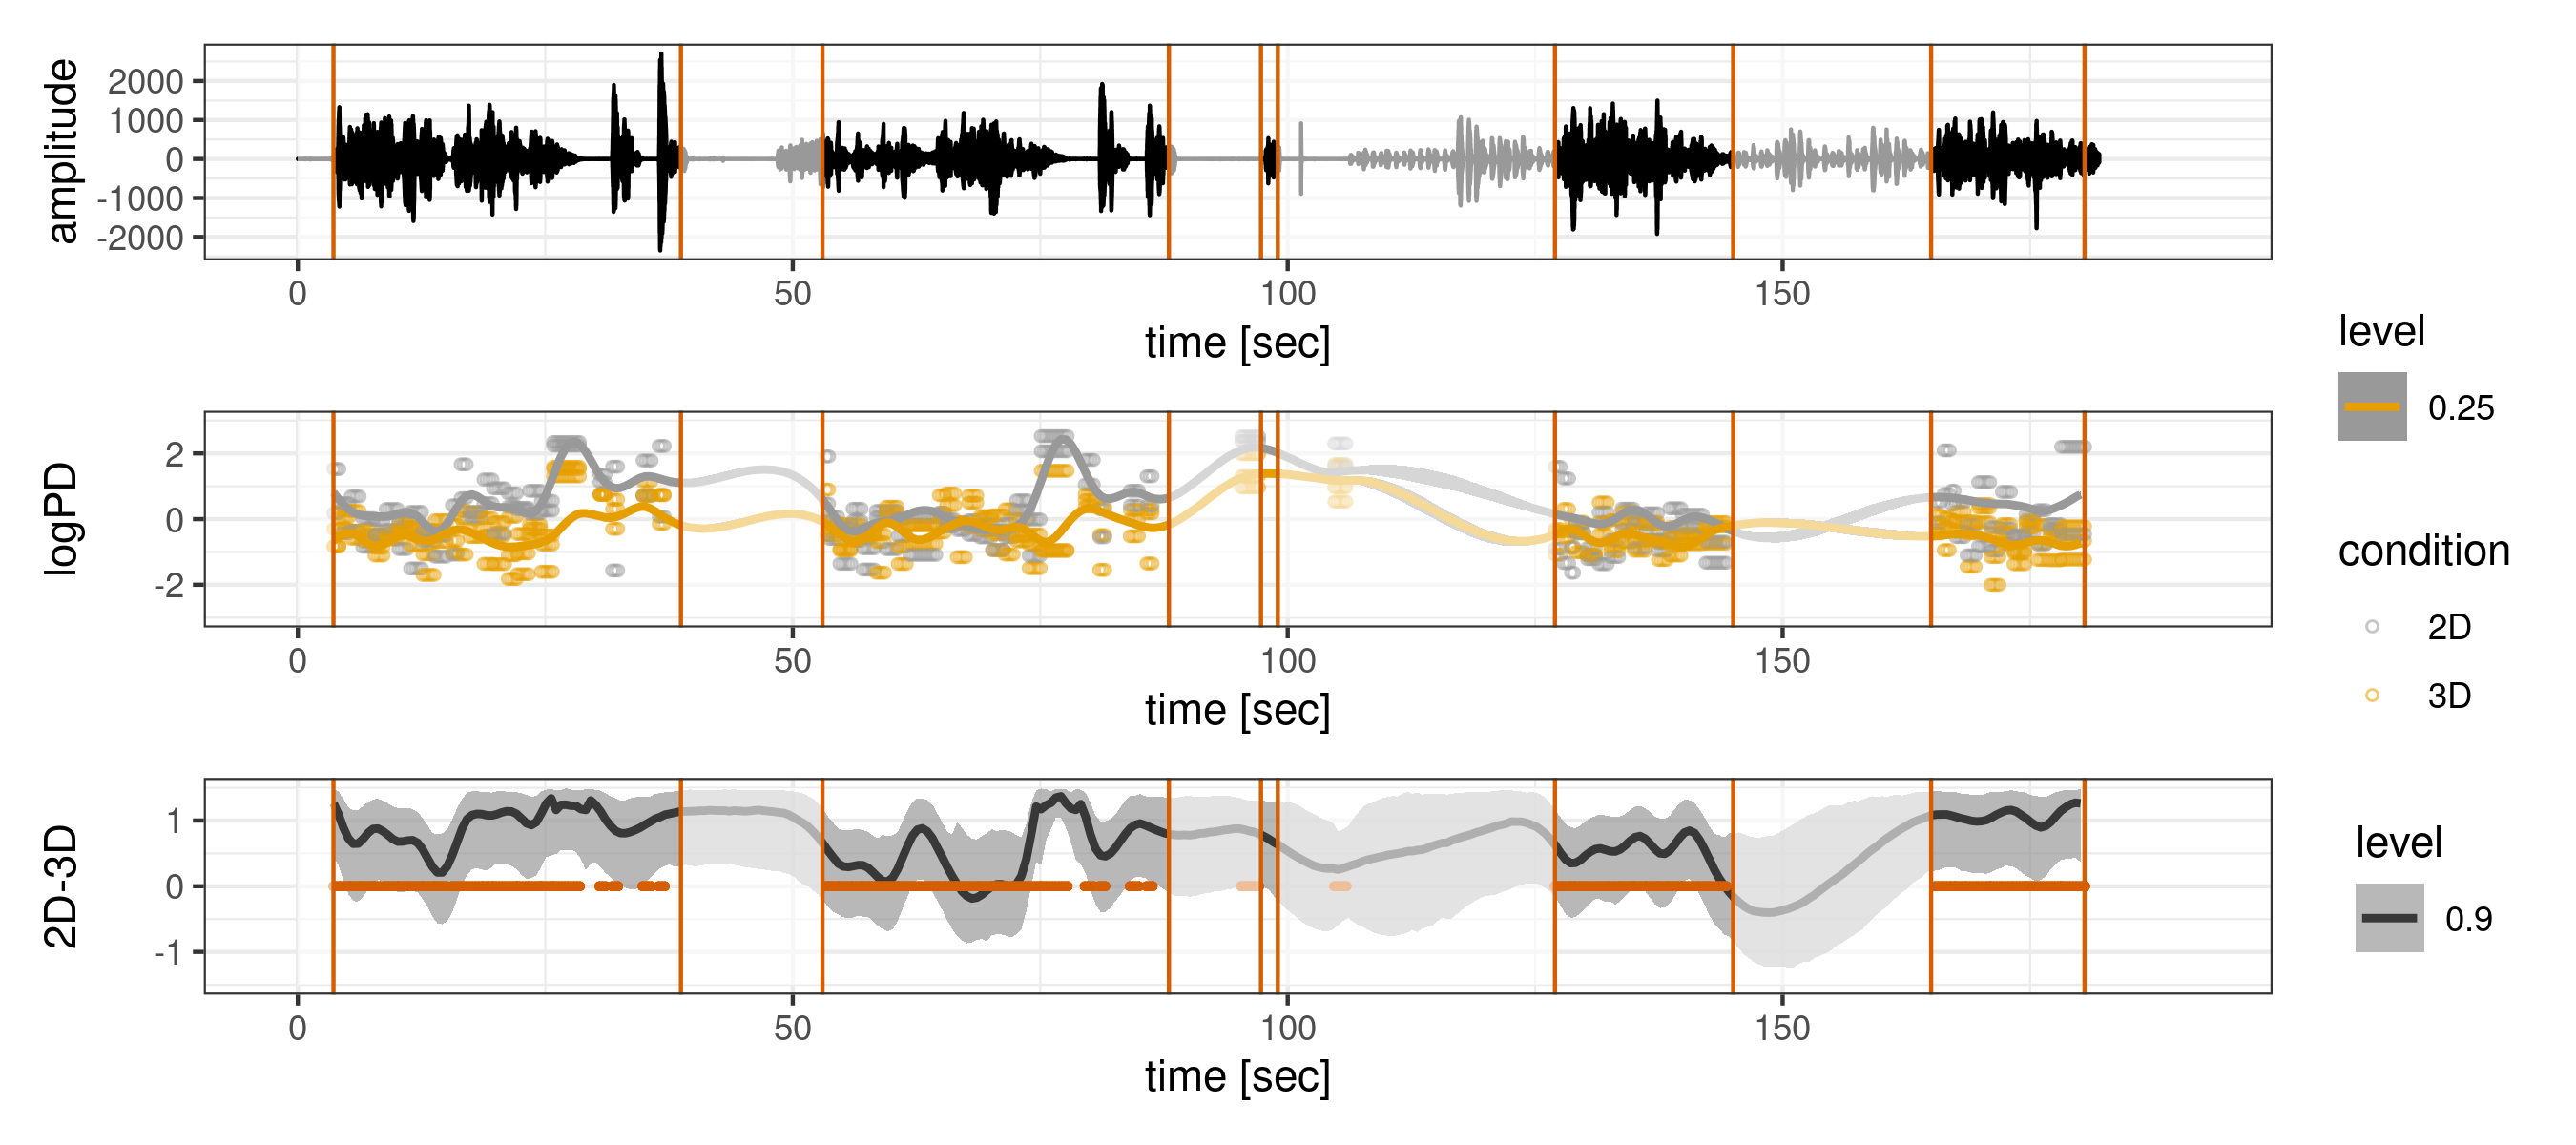
\includegraphics[width=1\linewidth]{Figures/chapViolinist_Diff_model_F1} 

}

\caption{Data of four pieces in two conditions}(\#fig:chapViolinist_PD_diff1)
\end{figure}

The top panel of figure @ref(fig:chapViolinist\_PD\_diff) shows the logPD of the bowing gestures of the 2D and 3D performances for all subjects and trials.
The smooths (2D in gray, 3D in ocre) show the \emph{posterior predictive distribution} calculated at each .5 seconds, of the mean and its uncertainty.
The figures shows 25\% of the distribution's probability mass (the critical interval at 25\%, or CI-25\%). Taking CI-90\% would result is more overlapping and less clear picture.
The vertical lines mark some relevant time points such as beginnings and endings of sections in the score, see figure @ref(fig:chapViolinist\_F1\_score). These marks are merely used as reference points for linking smooths to data.

The bottom panel of figure @ref(fig:chapViolinist\_PD\_diff) shows the \emph{posterior difference distribution}, calculated at each sample of time.
One such distribution is based on drawing a number (e.g., 100, or 1000) random samples from the two posterior predictive distributions, and adding the difference \(2D - 3D\) to a new distribution, called the \emph{posterior difference distribution}.
In this calculation, the entire probability mass is involved (rather than the CI-25\% shown in figure @ref(fig:chapViolinist\_PD\_diff)).
The band shows the \(2D-3D\) mean and its CI-90\%.
If, at a certain point in time, this gray band is completely above zero, then, there is a strong support for 2D being distinct from 3D, with higher logPD value.
If this gray band is completely below zero, then there is a strong support for 2D being different from 3D, with lower logPD value.
If it crosses zero, then it depends on how much of the probability mass is different from zero. If it is still 70\%, one could argue for a very weak trend, but 50\% would certainly indicate no difference.
In short, when the gray band is above zero it is possible to conclude that the student's bowing gestures are better lined up with the 3D teacher's bowing gestures.

It's fascinating to see this \emph{posterior difference distribution} changing over time.
To get an idea of what happens it is useful to look at the data in blocks:
a first block from 3 seconds to 40 seconds,
a second one from 53 to 90,
a third one from 127 to 145, and
a fourth one from 165 to 181.5.

First consider block one and two.
The end of these blocks is marked by short phrases followed by a long silence.
In both blocks, a sudden short peak appears at 25 and at 75 seconds, corresponding to the ending of a phrase (red vertical line) where longer notes are played.
The first block is almost everywhere significantly different, while the second block, except for the peak, is not significantly different and it even has a small downwards peak at about 63 seconds.

Next consider block three and four.
The third block shows 2D to be distinct from 3D, while the fourth block is even more distinct than the first block.
Overall, except for the second block, there is strong support for 2D being different from 3D.

The overall conclusion is that the student's alignment with the teacher, in terms of bowing gestures, works better in 3D than in 2D. At some time instances, especially when long notes are played at the ending of a block, the difference is suddenly more prominent. However, these peaks are not appearing in blocks three and four.

\hypertarget{second-piece-f2}{%
\subsection{Second piece (F2)}\label{second-piece-f2}}

In the \emph{posterior difference distribution} of the second piece
similar peaks are observed, indicating better alignment in 3D than 2D.
The alignment of short bowing gestures (starting at 45 s) is better in 3D.
Considering the high logPD values it seems that the task is difficult.

However, a first negative peak indicating that 2D is better is observed at
about 78 s. Then again a postive peak indicating that 3D is better at 113 s.
The final section (starting slightly before 150s) indicates a better alignment with 2D than 3D.

Overall, the picture seems to suggest that if the task is difficult, then 3D is in the advantage.

\begin{figure}

{\centering 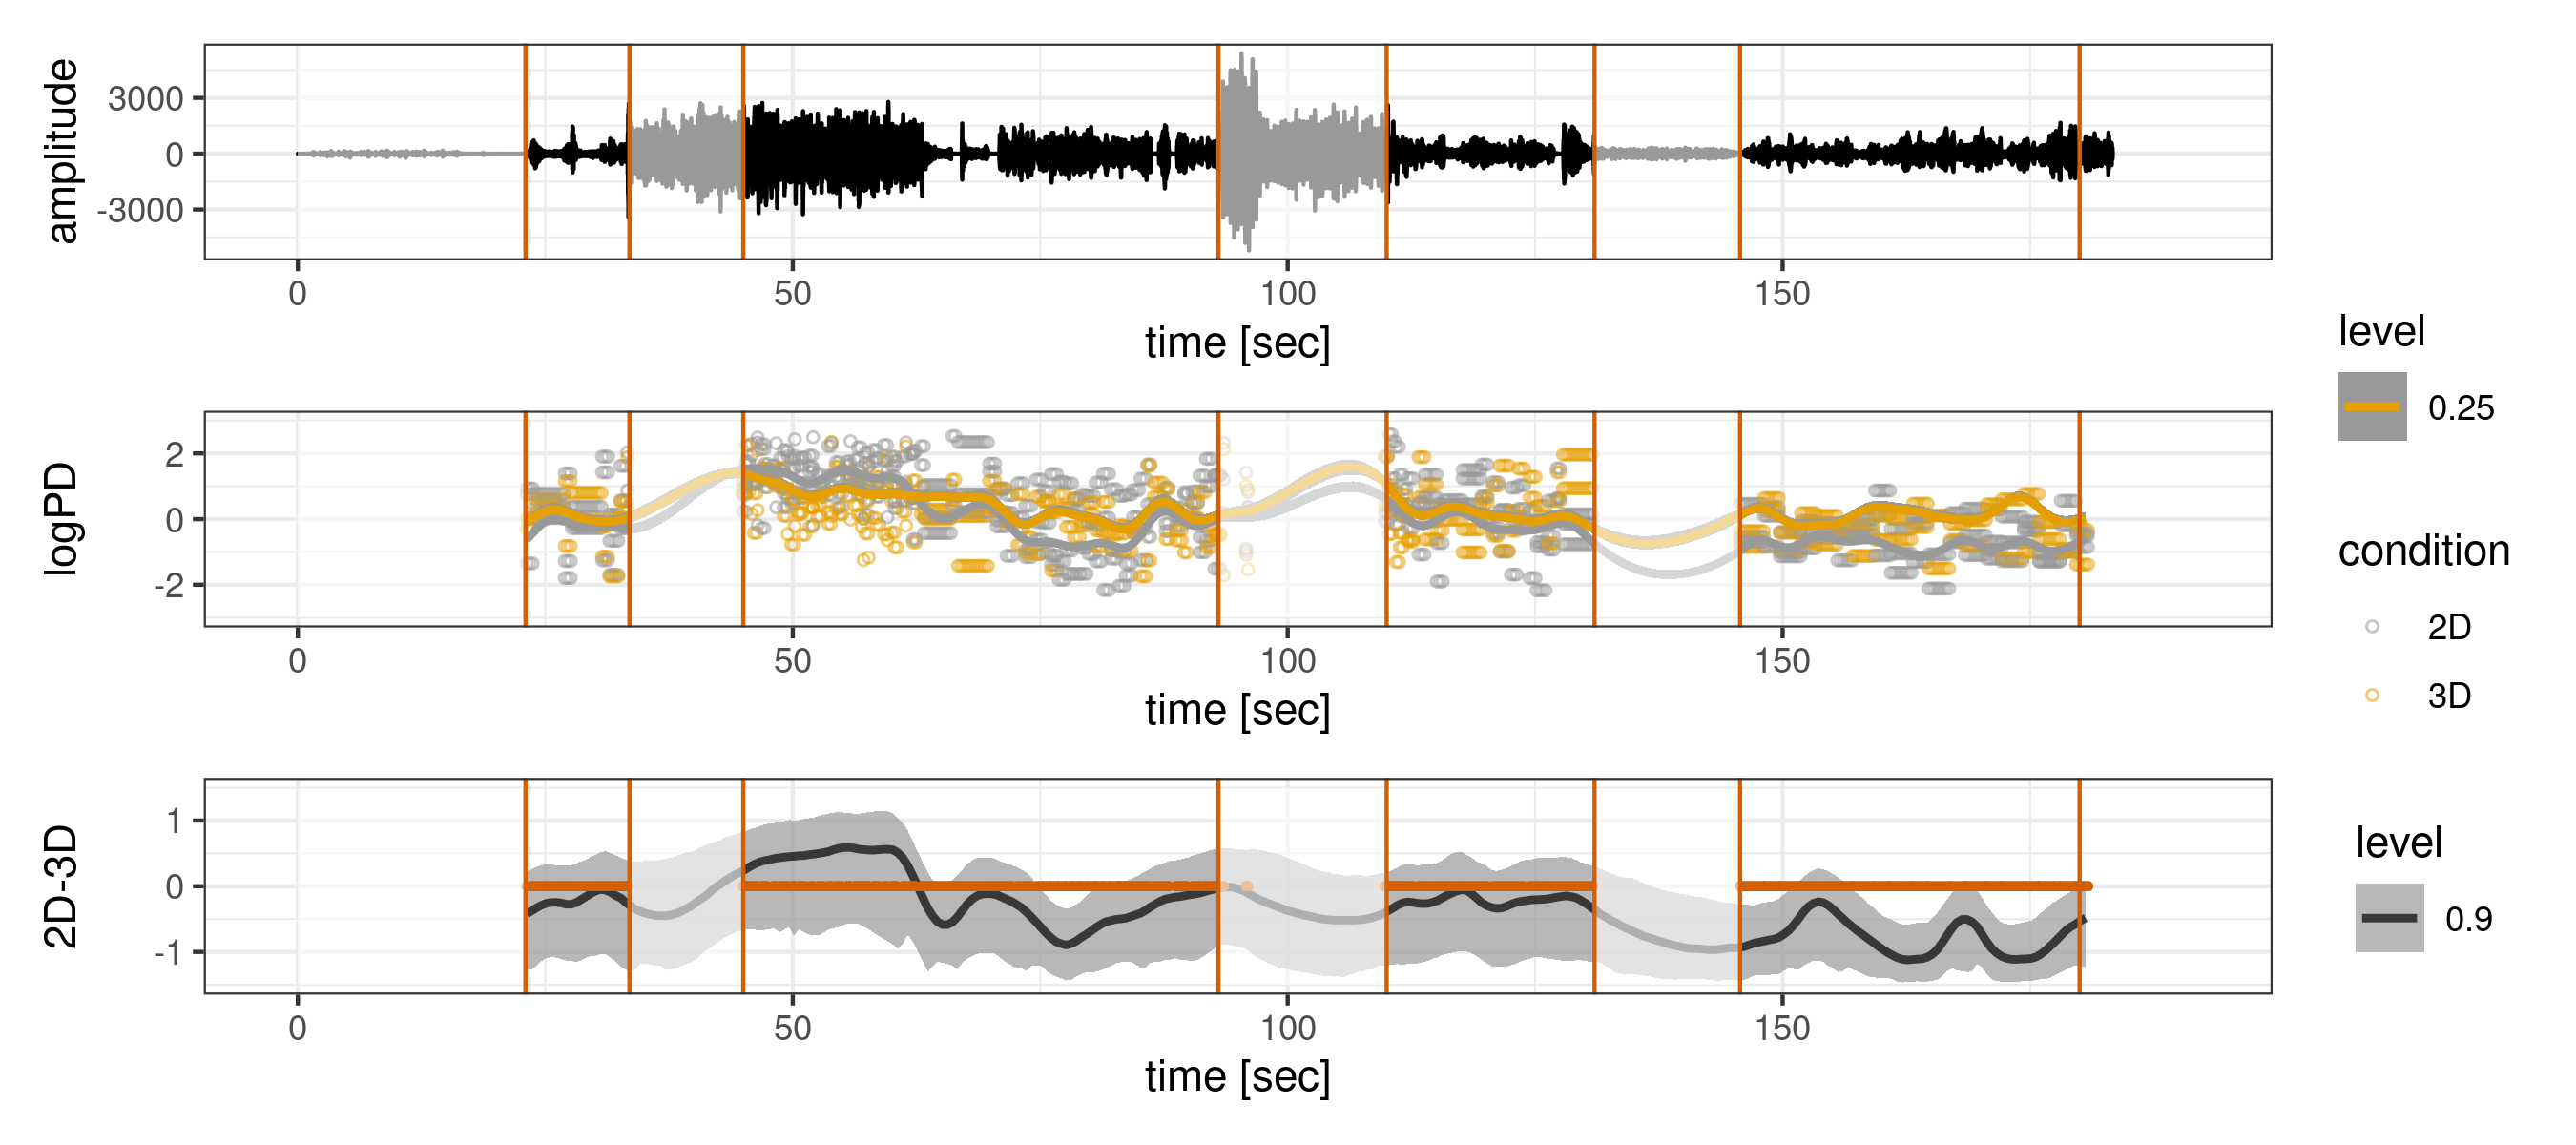
\includegraphics[width=1\linewidth]{Figures/chapViolinist_Diff_model_F2} 

}

\caption{Data of four pieces in two conditions}(\#fig:chapViolinist_PD_diff2)
\end{figure}

\begin{figure}
  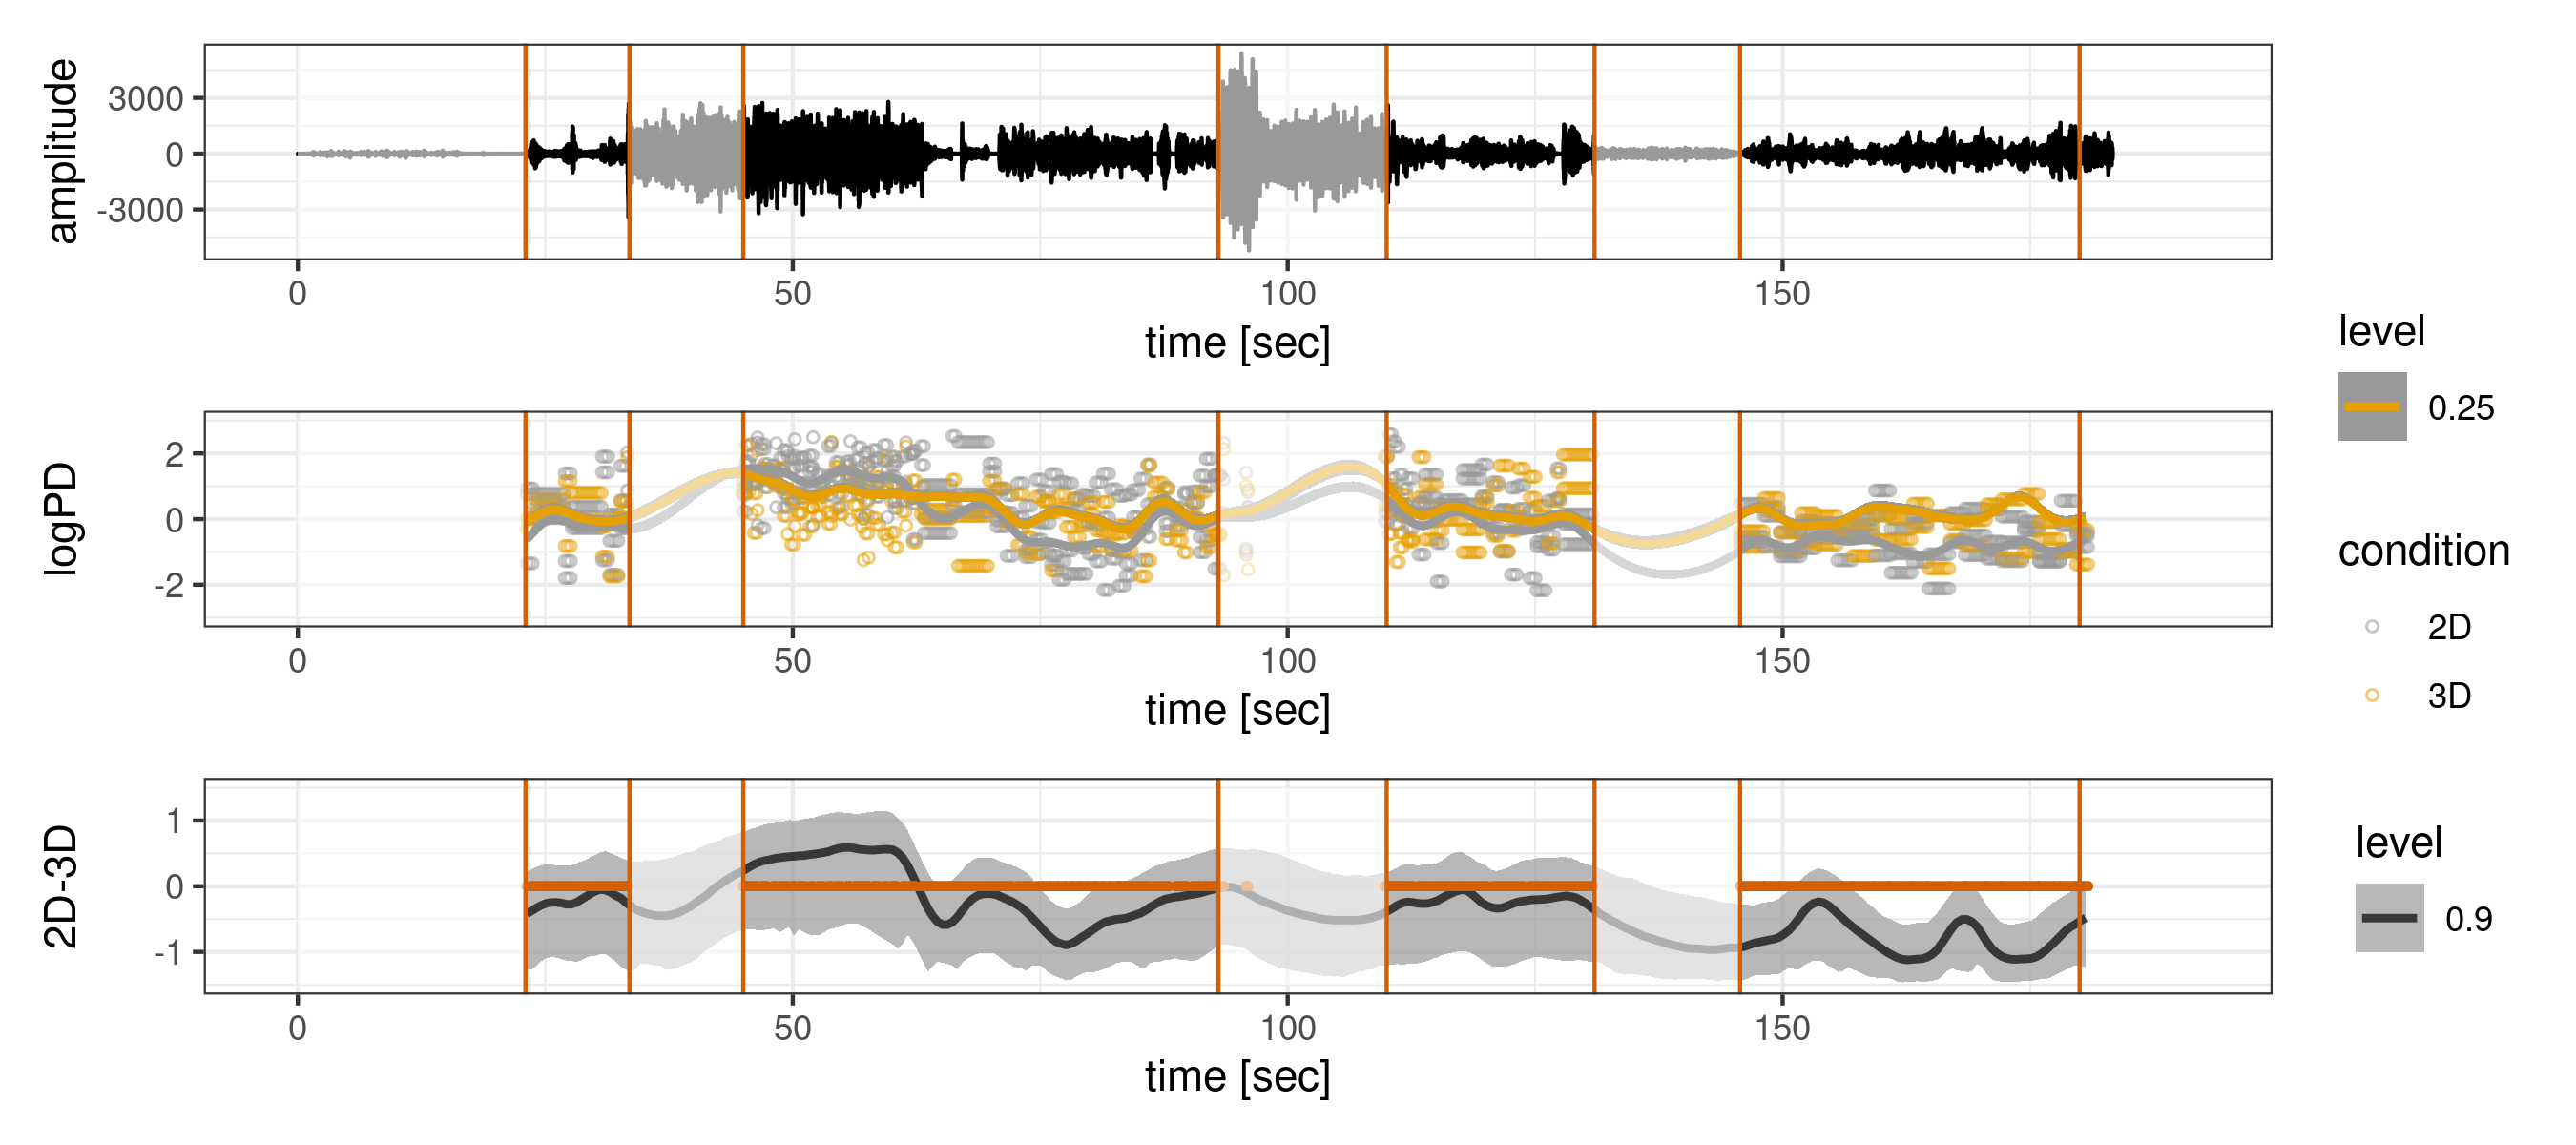
\includegraphics{"Figures/chapViolinist_Diff_model_F2.pdf"}
  \caption{This is a figure.}
\end{figure}

\hypertarget{chapEntrainment}{%
\chapter{Understanding two finger tappers being entrained}\label{chapEntrainment}}

Campo, A., Michałko, A., Van Kerrebroeck, B., Stajic, B., Pokric, M., and Leman, M. (2023a). The assessment of presence and performance in an AR environment for motor imitation learning: A case-study on violinists, Computers in Human Behavior, Volume 146, 2023, 107810, ISSN 0747-5632, \url{https://doi.org/10.1016/j.chb.2023.107810}.

Campo, A., Michałko, A., Van Kerrebroeck, B., and Leman, M. (2023b).
Dataset for the assessment of presence and performance in an augmented reality environment for motor imitation learning: A case-study on violinists. Data in Brief 51 109663.
\url{https://10.1016/j.chb.2023.107810}

Campo,A., Van Kerrebroeck, B., Leman, M. (2024).
MC-AR --- A software suite for comparative mocap analysis in an augmented reality environment
Software Impacts 19 100605. \url{https://doi.org/10.1016/j.dib.2023.109663}.

References

Bader, R. (Ed.). (2018). Springer handbook of systematic musicology. Springer.
Beltrán, M.I., Dudink, J., de Jong, T.M. et al.~Sensory-based interventions in the NICU: systematic review of effects on preterm brain development. Pediatr Res 92, 47--60 (2022).

Bonicco-Donato, D. (2016). Une archéologie de l'interaction. De David Hume à Erving Goffman. Paris: Vrin.

Clayton, M., Sager, R., \& Will, U. (2005). In time with the music: the concept of entrainment and its significance for ethnomusicology. In European meetings in ethnomusicology.(Vol. 11, pp.~1-82). Romanian Society for Ethnomusicology.

Collins, T., Tillmann, B., Barrett, F. S., Delbé, C., \& Janata, P. (2014). A combined model of sensory and cognitive representations underlying tonal expectations in music: from audio signals to behavior. Psychological review, 121(1), 33.

François C, Rodriguez-Fornells A, Teixidó M, Agut T, Bosch L. Attenuated brain responses to speech sounds in moderate preterm infants at term age. Dev Sci. 2021;24:e12990.

Godøy, R. I. (2003). Motor-mimetic music cognition. Leonardo, 36(4), 317-319.

Godøy, R. I. (2010). Gestural affordances of musical sound. In Musical Gestures (pp.~115-137). Routledge.

Goldin-Meadow, S. (2005). Hearing gesture: How our hands help us think. Harvard University Press.

Huron, D. (2008). Sweet anticipation: Music and the psychology of expectation. MIT press.

Kahneman, D. (2011). Thinking, fast and slow. Macmillan.

Koelsch, S., Vuust, P., \& Friston, K. (2019). Predictive processes and the peculiar case of music. Trends in cognitive sciences, 23(1), 63-77.

Langner, G. D. (2015). The neural code of pitch and harmony. Cambridge University Press.

Leman, M. (2007). Embodied music cognition and mediation technology. MIT press.

Leman, M. (2016). The expressive moment: How interaction (with music) shapes human empowerment. MIT press.

Lorenzoni, V., Van den Berghe, P., Maes, P. J., De Bie, T., De Clercq, D., \& Leman, M. (2019a). Design and validation of an auditory biofeedback system for modification of running parameters. Journal on Multimodal User Interfaces, 13(3), 167-180.

Lorenzoni, V., Staley, J., Marchant, T., Onderdijk, K. E., Maes, P. J., \& Leman, M. (2019b). The sound instructor: a music-based biofeedback system for improving weightlifting technique. Plos one, 14(8), e0220915.

Maes, P. J., Leman, M., Palmer, C., \& Wanderley, M. M. (2014). Action-based effects on music perception. Frontiers in psychology, 4, 1008.

Maes, P. J., Lorenzoni, V., \& Six, J. (2019). The SoundBike: musical sonification strategies to enhance cyclists' spontaneous synchronization to external music. Journal on Multimodal User Interfaces, 13(3), 155-166.

Malloch, S. (1999). Mothers and infants and communicative musicality. Musicae Scientiae special issue 1999-2000, 29-57.

McGowan, T., \& Delafield-Butt, J. (2022). Narrative as co-regulation: A review of embodied narrative in infant development. Infant Behavior and Development, 68, 101747.

Moens, B., Muller, C., Van Noorden, L., Franěk, M., Celie, B., Boone, J., \ldots{} \& Leman, M. (2014). Encouraging spontaneous synchronisation with D-Jogger, an adaptive music player that aligns movement and music. PloS one, 9(12), e114234.

Moumdjian, L., Moens, B., Maes, P. J., Van Nieuwenhoven, J., Van Wijmeersch, B., Leman, M., \& Feys, P. (2019). Walking to music and metronome at various tempi in persons with multiple sclerosis: a basis for rehabilitation. Neurorehabilitation and neural repair, 33(6), 464-475.

Phillips-Silver, J., \& Keller, P. E. (2012). Searching for roots of entrainment and joint action in early musical interactions. Frontiers in human neuroscience, 6, 26.

Schiavio, A., Maes, P. J., \& van der Schyff, D. (2022). The dynamics of musical participation. Musicae Scientiae, 26(3), 604-626.

Sears, D. R., Pearce, M. T., Spitzer, J., Caplin, W. E., \& McAdams, S. (2019). Expectations for tonal cadences: Sensory and cognitive priming effects. Quarterly Journal of Experimental Psychology, 72(6), 1422--1438. \url{https://doi.org/10.1177/1747021818814472}

Seth, Anil K. The cybernetic Bayesian brain. Open mind. Frankfurt am Main: MIND Group, 2014.

Schneider, A. (2018a). Pitch and pitch perception. In Springer Handbook of Systematic Musicology (pp.~605-686). Springer, Berlin, Heidelberg.

Schneider, A. (2018b). Perception of timbre and sound color. In Springer Handbook of Systematic Musicology (pp.~687-725). Springer, Berlin, Heidelberg.

Trehub, S. (2013). Communication, Music, and Language in Infancy. In ``Language, Music, and the Brain,'' edited by Michael A. Arbib. Strüngmann Forum Reports, vol.~10. MIT Press.

Trevarthen, C., \& Aitken, K. J. (2001). Infant intersubjectivity: Research, theory, and clinical applications. The Journal of Child Psychology and Psychiatry and Allied Disciplines, 42(1), 3-48.

Trevarthen, C. (2008). The musical art of infant conversation: Narrating in the time of sympathetic experience, without rational interpretation, before words. Musicae Scientiae, 12(1\_suppl), 15-46.

Trost, W. J., Labbé, C., \& Grandjean, D. (2017). Rhythmic entrainment as a musical affect induction mechanism. Neuropsychologia, 96, 96-110.

Van den Berghe, P., Lorenzoni, V., Derie, R., Six, J., Gerlo, J., Leman, M., \& De Clercq, D. (2021). Music-based biofeedback to reduce tibial shock in over-ground running: A proof-of-concept study. Scientific reports, 11(1), 1-12.

Van den Berghe, P., Derie, R., Bauwens, P., Gerlo, J., Segers, V., Leman, M., \& De Clercq, D. (2022). Reducing the peak tibial acceleration of running by music‐based biofeedback: A quasi‐randomized controlled trial. Scandinavian Journal of Medicine \& Science in Sports, 32(4), 698-709.

Van Puyvelde, M., Loots, G., Vinck, B., De Coster, L., Matthijs, L., Mouvet, K., \& Pattyn, N. (2013). The interplay between tonal synchrony and social engagement in mother--infant interaction. Infancy, 18(5), 849-872.

\hypertarget{chapAugHumanities}{%
\chapter{Augmented humanities}\label{chapAugHumanities}}

\begin{Shaded}
\begin{Highlighting}[]
\NormalTok{knitr}\SpecialCharTok{::}\NormalTok{opts\_chunk}\SpecialCharTok{$}\FunctionTok{set}\NormalTok{(}\AttributeTok{class.source =} \StringTok{"watch{-}out"}\NormalTok{)}
\end{Highlighting}
\end{Shaded}

The shift from \emph{SR} to \emph{interaction}, and from \emph{measurement} to \emph{modelling} defines a major development in modern musicology. This development has far-reaching consequences for musicology, as well as for the umbrella disciplines that is called: the humanities.
Let us have a very brief look at this development.
After that here will be time enough to narrow down our ambitious, and concentrate our thoughts on the statistical processing of time-varying data, or at least offer a small contribution to the huge challenge it poses.

\hypertarget{the-paradigm-shift}{%
\section{The paradigm shift}\label{the-paradigm-shift}}

There was a time that studies in music perception required listener's to listen to a musical pattern, when then responded to that pattern with yes/no, a scoring, or perhaps a reaction time. In these studies, stimulus comes first and the response is an event.
However, with studies in music performance this concept changed dramatically.
Rather than \emph{stimulus-response (SR)}, the prevailing paradigm is \emph{interactive}, with studies focusing on actions during a task, preferably in a context.

The challenges of this paradigm are technical.
First, consider the challenge of \emph{data-acquisition}. As data-acquisition happens during the presentation of the stimulus multiple recording devices are needed, such as audio, video, motion caption systems, eye-tracking, EEG-recordings and so on. These devices generate information streams that need to be assembled and synchronized up to the sub-millisecond level of accuracy. It requires sophisticated machinery for time-stamping multimedia data streams, storing them, and have flexible accessibility afterwards.
Many labs meanwhile can deal with multimedia data streams.
Second, consider the challenge of \emph{data modelling}. One we have multimedia data streams, we need sophisticated tools for feature extraction, classification and machine learning. Ultimately, the goal is to use knowledge about human performance and use it to the benefit of our society. The study of human perfmance then contributes to a larger framework of human activity and human collaboration.
But what sort of activity is this and what is the larger framework of that study?
Musicology used to be part of the humanities but the above shift in paragm has challenged the humanities and, meanwhile, musicology became of on the disciplines that transformed the humanities.
This book should be conceived as contribution to that transformation.

\hypertarget{the-humanities}{%
\section{The humanities}\label{the-humanities}}

The ``humanities'' include a wide range of disciplines that seek to understand various aspects of human activities and artifacts through philosophical clarification and analysis.
The traditional methodology revolves around the use of qualitative means to identify, clarify and analyze phenomena. However, this traditional methodology has evolved and included methods for data handling, as well as methods that probe deeper levels of the phenomena.

The humanities produced large amounts of data, and many studies currently apply quantitative analysis methods employed in other scientific disciplines to these data.
One example is my art history colleague's use of ``event history analysis'' to describe the collective biographies of Antwerp artists between 1490 and 1530.
{[}{[}{[}(Martens, 2004, Antwerp Painters: Their Markets and Their Networks). {]}{]}{]}

Likewise, in many areas of the humanities, phenomenological understanding has been enhanced by incorporating levels of understanding based on insights from other disciplines. The same history collegue uses radiographic techniques for scanning paintings, thereby uncovering levels of the painting that cannot be observed by the naked eye, leading to new interpretations and a deeper understanding of the painting.
{[}{[}{[}XXXXXXXX{]}{]}{]}
Many examples can be given in the domain of archeology, history, and linguistics to mention but a few of the core disciplines in the humanities.

\hypertarget{the-augmented-humanities}{%
\section{The augmented humanities}\label{the-augmented-humanities}}

Musicology has always been at the foreground of this transformation to ``augmentation''.
Already in the 19th century, the work Hermann von Helmholtz had a significant impact on musicology because he aimed at understanding tonal perception by explaining it from an acoustic and human physiological perspective. It expanded musicology with new insights that offered deeper levels of understanding the phenomenon of tonality.
With advances in cognitive science and increased interest in electronic music production in the 1960s, methods of sound manipulation became more accessible. When computer platforms emerged in the 1990s, musicology was already at the forefront of experimentation with computational modelling and early forms of machine learning, as a new tool to understand music.
It was shocking new for the humanities and questions could be heard whether this research still belonged to the ``humanities''?

Gradually, however, this new approach took shape and moved towards a specific theory of human interaction with music, which considered the study of musical signals, body movement and meaning-making as interrelated aspects of a holistic approach, fundamentally rooted in the humanities. This perspective also included new technologies that enable measurements beyond what can be seen with the naked eye.

By the beginning of the twentieth century, a new form of understanding emerged, closely related to approaches from psychology, neuroscience, and engineering, but still rooted in the humanities. This understanding was based on the idea that insight in a phenomenon can be proactive in nature, meaning that it can predict the effects of actions rather than simply describe observed phenomena (being the primary occupation of the traditional humanities).
For example, controlled experiments and predictions of effects suggest that rhythmic stimulation improves the pace of people with Parkinson's disease, or that music-based biofeedback reduces peak impacts by 28\% in runners (XXXX examination). Obviously, in other domains of the humanities we observe a similar trend. This proactive approach implied prediction of new historical evidence due to discovered overpainting on a painting, or prediction of artifacts in undergrounds. In archaeogenetics, proactive thinking is currently revolutionizing the time-line of archeology, providing many new insights in understanding human evolution and development.

As we all know, ``event history analysis'' began as ``survival analysis'' in biomedical research.
Its use in the humanities is a classic example of methodological augmentation, which suggests the term ``augmented humanities''.
Likewise, advances in neuroscience and biology contribute to the understanding of meaningful activity, for example in art and religion, by pointing to brain mechanisms, hormones and neurotransmitter systems (e.g.~the dopaminergic system). Although there is a necessary qualitative understanding of the cultural context in which meaning-making activities occur, a deeper understanding, even if only partial, can shed new light on the phenomenon and strengthen its qualitative description.

In the past decades, the \emph{augmented humanities} became a partner at equal level with other modern sciences such as engineering, neuroscience, and neurobiology. Be it the Raman spectroscopy of old paintings in art history, 3D scanning of ancient buildings in archeology, genetics in studies of human migration in history, or AI applied to natural language processing in linguistics, humanities gradually became a partner of value for other sciences.

\hypertarget{key-features-of-augmented-humanities}{%
\section{Key features of augmented humanities}\label{key-features-of-augmented-humanities}}

Augmented humanities got enriched by new methods from other sciences.
- recording technologies
- data modelling techniques
- representation tools

\hypertarget{chapDriftingMetronomes}{%
\chapter{Drifting metronomes paradigm}\label{chapDriftingMetronomes}}

\hypertarget{footnotes-and-citations}{%
\chapter{Footnotes and citations}\label{footnotes-and-citations}}

\hypertarget{footnotes}{%
\section{Footnotes}\label{footnotes}}

Footnotes are put inside the square brackets after a caret \texttt{\^{}{[}{]}}. Like this one \footnote{This is a footnote.}.

\hypertarget{citations}{%
\section{Citations}\label{citations}}

Reference items in your bibliography file(s) using \texttt{@key}.

For example, we are using the \textbf{bookdown} package \citep{R-bookdown} (check out the last code chunk in index.Rmd to see how this citation key was added) in this sample book, which was built on top of R Markdown and \textbf{knitr} \citep{xie2015} (this citation was added manually in an external file book.bib).
Note that the \texttt{.bib} files need to be listed in the index.Rmd with the YAML \texttt{bibliography} key.

The RStudio Visual Markdown Editor can also make it easier to insert citations: \url{https://rstudio.github.io/visual-markdown-editing/\#/citations}

\hypertarget{blocks}{%
\chapter{Blocks}\label{blocks}}

\hypertarget{equations}{%
\section{Equations}\label{equations}}

Here is an equation.

\begin{equation} 
  f\left(k\right) = \binom{n}{k} p^k\left(1-p\right)^{n-k}
  \label{eq:binom}
\end{equation}

You may refer to using \texttt{\textbackslash{}@ref(eq:binom)}, like see Equation \eqref{eq:binom}.

\hypertarget{theorems-and-proofs}{%
\section{Theorems and proofs}\label{theorems-and-proofs}}

Labeled theorems can be referenced in text using \texttt{\textbackslash{}@ref(thm:tri)}, for example, check out this smart theorem \ref{thm:tri}.

\begin{theorem}
\protect\hypertarget{thm:tri}{}\label{thm:tri}For a right triangle, if \(c\) denotes the \emph{length} of the hypotenuse
and \(a\) and \(b\) denote the lengths of the \textbf{other} two sides, we have
\[a^2 + b^2 = c^2\]
\end{theorem}

Read more here \url{https://bookdown.org/yihui/bookdown/markdown-extensions-by-bookdown.html}.

\hypertarget{callout-blocks}{%
\section{Callout blocks}\label{callout-blocks}}

The R Markdown Cookbook provides more help on how to use custom blocks to design your own callouts: \url{https://bookdown.org/yihui/rmarkdown-cookbook/custom-blocks.html}

\hypertarget{sharing-your-book}{%
\chapter{Sharing your book}\label{sharing-your-book}}

\hypertarget{publishing}{%
\section{Publishing}\label{publishing}}

HTML books can be published online, see: \url{https://bookdown.org/yihui/bookdown/publishing.html}

\hypertarget{pages}{%
\section{404 pages}\label{pages}}

By default, users will be directed to a 404 page if they try to access a webpage that cannot be found. If you'd like to customize your 404 page instead of using the default, you may add either a \texttt{\_404.Rmd} or \texttt{\_404.md} file to your project root and use code and/or Markdown syntax.

\hypertarget{metadata-for-sharing}{%
\section{Metadata for sharing}\label{metadata-for-sharing}}

Bookdown HTML books will provide HTML metadata for social sharing on platforms like Twitter, Facebook, and LinkedIn, using information you provide in the \texttt{index.Rmd} YAML. To setup, set the \texttt{url} for your book and the path to your \texttt{cover-image} file. Your book's \texttt{title} and \texttt{description} are also used.

This \texttt{gitbook} uses the same social sharing data across all chapters in your book- all links shared will look the same.

Specify your book's source repository on GitHub using the \texttt{edit} key under the configuration options in the \texttt{\_output.yml} file, which allows users to suggest an edit by linking to a chapter's source file.

Read more about the features of this output format here:

\url{https://pkgs.rstudio.com/bookdown/reference/gitbook.html}

Or use:

\begin{Shaded}
\begin{Highlighting}[]
\NormalTok{?bookdown}\SpecialCharTok{::}\NormalTok{gitbook}
\end{Highlighting}
\end{Shaded}

bookdown::render\_book(``index.Rmd'', ``bookdown::gitbook'')
bookdown::render\_book(``index.Rmd'', ``bookdown::pdf\_book'')

  \bibliography{book.bib,packages.bib}

\end{document}
